\documentclass[11pt,a4paper]{article}
\usepackage[margin=2.3cm]{geometry}
\usepackage{amsmath,amssymb}
\usepackage{booktabs}
\usepackage{xcolor}
\usepackage{graphicx}
\usepackage{tikz}
\usetikzlibrary{arrows.meta,positioning,calc}
\usepackage[colorlinks=true,linkcolor=blue!50!black]{hyperref}
\graphicspath{{figs/}{../exp_data/}}

\title{Green preconditioner corrected for Dirichlet conditions}
\author{muFFTTO, \texttt{experiments/linear\_elastic\_mesh\_study}}
\date{23 October 2026, updated 26 October 2026}

\begin{document}
\maketitle

\section*{Setting}

Notation as in the double-Green paper: $\mathbf{K}(\mathbb{C}) = \mathbf{B}^{\top}\mathbf{W}\mathbb{C}\mathbf{B}$ is the
stiffness matrix of the material $\mathbb{C} = \operatorname{diag}(\mathbb{C}_q)$, $n$ the number of nodal unknowns,
$\mathbb{C}_0$ the constant reference material, and
\[
  \mathbf{G}_0 = \bigl(\mathbf{K}(\mathbb{C}_0)\bigr)^{-1} \quad \text{on } V_0
\]
the Green operator, applied by FFT with the zero frequency omitted. Write $\mathbf{K}_0 = \mathbf{K}(\mathbb{C}_0)$ and
$\mathbf{K} = \mathbf{K}(\mathbb{C})$.

\paragraph{Kernel.} $\mathbf{K}_0$ is singular. Its kernel is spanned by the $d$ rigid translations,
\[
  \mathbf{N} \in \mathbb{R}^{n\times d}, \qquad \mathbf{N}_{:,i} = \mathbf{e}_i \otimes \mathbf{1},
\]
and $\mathbf{G}_0$ satisfies $\mathbf{G}_0\mathbf{N} = \mathbf{0}$ and $\mathbf{K}_0\mathbf{G}_0\mathbf{v} = \mathbf{v}$ for
all $\mathbf{v}$ with $\mathbf{N}^{\top}\mathbf{v} = \mathbf{0}$.

\paragraph{Dirichlet conditions.} Let $m$ dofs be fixed, and let $\mathbf{P} \in \mathbb{R}^{n\times n}$ be the projection onto
them (diagonal, 1 at the fixed dofs and 0 elsewhere). $\mathbf{Q} = \mathbf{I} - \mathbf{P}$ is the projection onto the free
dofs. With the prescribed values lifted to the right-hand side, the problem is
\[
  \mathbf{Q}\mathbf{K}\mathbf{Q}\,\mathbf{u} = \mathbf{Q}\mathbf{f}, \qquad \mathbf{P}\mathbf{u} = \mathbf{0}.
\]
We assume that the fixed dofs remove the translations, i.e.\ $\mathbf{P}\mathbf{N}$ has full column rank $d$. Then
$\mathbf{Q}\mathbf{K}_0\mathbf{Q}$ is positive definite on the free dofs.

\section*{Plain (projected) Green}

The preconditioner used so far is
\[
  \mathbf{M}_{\mathrm{G}} = \mathbf{Q}\,\mathbf{G}_0\,\mathbf{Q}.
\]
It is \emph{not} the inverse of the constrained reference operator: in general
$\mathbf{Q}\mathbf{G}_0\mathbf{Q} \neq (\mathbf{Q}\mathbf{K}_0\mathbf{Q})^{-1}$ on the free dofs. The bound
$\lambda_{\max}(\mathbf{M}_{\mathrm{G}}\mathbf{K}) \le 1$ for $\mathbb{C}_q \le \mathbb{C}_0$ is therefore lost. Measured:
$\lambda_{\max} \approx 0.6\sqrt{k\,n_H}$ for $k$ fixed nodes, i.e.\ $\propto 1/h$ for a clamped face.

\section*{Corrected Green}

\paragraph{Definition.} The corrected preconditioner is the exact inverse of the constrained reference problem,
\[
  \mathbf{M}_{\mathrm{GD}} = \bigl(\mathbf{Q}\mathbf{K}_0\mathbf{Q}\bigr)^{-1} \quad \text{on the free dofs}.
\]
Applying it to a residual $\mathbf{r}$ (with $\mathbf{P}\mathbf{r} = \mathbf{0}$) means solving the saddle-point problem
\[
  \begin{bmatrix} \mathbf{K}_0 & \mathbf{P} \\ \mathbf{P} & \mathbf{0} \end{bmatrix}
  \begin{bmatrix} \mathbf{z} \\ \boldsymbol{\lambda} \end{bmatrix}
  =
  \begin{bmatrix} \mathbf{r} \\ \mathbf{0} \end{bmatrix},
\]
where $\boldsymbol{\lambda} = \mathbf{P}\boldsymbol{\lambda}$ are the reaction forces of the reference problem at the fixed dofs.

\paragraph{Solution with the Green operator.} The first row, $\mathbf{K}_0\mathbf{z} = \mathbf{r} - \boldsymbol{\lambda}$, is
solvable if and only if the right-hand side does no work on the translations,
\begin{equation}
  \mathbf{N}^{\top}\bigl(\mathbf{r} - \boldsymbol{\lambda}\bigr) = \mathbf{0},
  \label{eq:compat}
\end{equation}
and then
\begin{equation}
  \mathbf{z} = \mathbf{G}_0\bigl(\mathbf{r} - \boldsymbol{\lambda}\bigr) + \mathbf{N}\boldsymbol{\alpha},
  \qquad \boldsymbol{\alpha} \in \mathbb{R}^{d}.
  \label{eq:z}
\end{equation}
The second row, $\mathbf{P}\mathbf{z} = \mathbf{0}$, and \eqref{eq:compat} give a small system for
$(\boldsymbol{\lambda}, \boldsymbol{\alpha})$:
\begin{equation}
  \begin{bmatrix} \mathbf{S} & \mathbf{P}\mathbf{N} \\ \mathbf{N}^{\top}\mathbf{P} & \mathbf{0} \end{bmatrix}
  \begin{bmatrix} \boldsymbol{\lambda} \\ -\boldsymbol{\alpha} \end{bmatrix}
  =
  \begin{bmatrix} \mathbf{P}\mathbf{G}_0\mathbf{r} \\ \mathbf{N}^{\top}\mathbf{r} \end{bmatrix},
  \qquad
  \mathbf{S} = \mathbf{P}\mathbf{G}_0\mathbf{P} \quad (\text{an } m\times m \text{ block on the range of } \mathbf{P}).
  \label{eq:capacitance}
\end{equation}
$\mathbf{S}$ is the Green operator restricted to the fixed dofs (the \emph{capacitance matrix}). It is symmetric
positive definite: for $\mathbf{y} = \mathbf{P}\mathbf{y} \neq \mathbf{0}$, $\mathbf{y}^{\top}\mathbf{S}\mathbf{y} =
\mathbf{y}^{\top}\mathbf{G}_0\mathbf{y} = 0$ would require $\mathbf{y}$ to be a translation, which is impossible unless all dofs are fixed. With
$\operatorname{rank}(\mathbf{P}\mathbf{N}) = d$, the bordered $(m+d)\times(m+d)$ matrix in \eqref{eq:capacitance} is
nonsingular.

\paragraph{Without the kernel.} If $\mathbf{K}_0$ were regular, \eqref{eq:z}--\eqref{eq:capacitance} reduce to the
Woodbury form
\[
  \mathbf{M}_{\mathrm{GD}} = \mathbf{G}_0 - \mathbf{G}_0\mathbf{P}\,\mathbf{S}^{-1}\mathbf{P}\mathbf{G}_0 \quad (\mathbf{S}^{-1} \text{ on the range of } \mathbf{P}).
\]
The bordering by $\mathbf{N}$ is what is needed because $\mathbf{G}_0$ omits the zero frequency.

\section*{Algorithm}

\paragraph{Setup (once).}
\begin{enumerate}
  \item For $j = 1,\dots,m$: apply $\mathbf{G}_0$ to the unit vector $\mathbf{e}_j$ of the $j$-th fixed dof and keep
        its values at the fixed dofs, $\mathbf{S}\mathbf{e}_j = \mathbf{P}\mathbf{G}_0\mathbf{e}_j$ ($m$ Green applications).
  \item Assemble the bordered matrix of \eqref{eq:capacitance} and factorize it ($(m+d)^3/3$ flops).
\end{enumerate}

\paragraph{Application $\mathbf{z} = \mathbf{M}_{\mathrm{GD}}\mathbf{r}$ (every CG iteration).}
\begin{enumerate}
  \item $\mathbf{y} = \mathbf{G}_0\mathbf{r}$ \hfill (Green application 1)
  \item solve \eqref{eq:capacitance} with the right-hand side $(\mathbf{P}\mathbf{y},\, \mathbf{N}^{\top}\mathbf{r})$
        for $(\boldsymbol{\lambda}, -\boldsymbol{\alpha})$
  \item $\mathbf{z} = \mathbf{G}_0(\mathbf{r} - \boldsymbol{\lambda}) + \mathbf{N}\boldsymbol{\alpha}$
        \hfill (Green application 2)
  \item $\mathbf{P}\mathbf{z} = \mathbf{0}$ holds by construction; set it exactly to remove round-off.
\end{enumerate}
One CG iteration costs two Green applications instead of one. The second can be avoided by storing
$\mathbf{G}_0\mathbf{P}$ (its $m$ nonzero columns, $n\times m$ numbers), since $\mathbf{G}_0(\mathbf{r} -
\boldsymbol{\lambda}) = \mathbf{y} - (\mathbf{G}_0\mathbf{P})\boldsymbol{\lambda}$; that trades memory for one FFT pair.

\section*{Properties}

\begin{itemize}
  \item \textbf{Exact for the reference.} If $\mathbb{C}_q = \mathbb{C}_0$ everywhere, then
        $\mathbf{M}_{\mathrm{GD}}\mathbf{Q}\mathbf{K}\mathbf{Q} = \mathbf{I}$ on the free dofs, for any set of fixed dofs.
  \item \textbf{Upper bound restored.} If $\mathbb{C}_q \le \mathbb{C}_0$ at every quadrature point (void included,
        $\mathbb{C}_q = 0$), then $\mathbf{Q}\mathbf{K}\mathbf{Q} \le \mathbf{Q}\mathbf{K}_0\mathbf{Q}$ on the free dofs, and hence
        \[
          \lambda_{\max}\bigl(\mathbf{M}_{\mathrm{GD}}\,\mathbf{Q}\mathbf{K}\mathbf{Q}\bigr) \le 1 ,
        \]
        independently of the number and position of the fixed dofs and of $h$.
  \item \textbf{Lower end.} $\lambda_{\min}$ is the smallest ratio of the energy in the real material to the energy in
        the constrained reference over the whole cell. As without Dirichlet conditions, it is set by the geometry and
        the void thickness, and is independent of $h$ when the void has a fixed physical thickness.
  \item \textbf{Same solution.} Only the preconditioner changes; the system and its solution do not.
\end{itemize}

\section*{Results}

Cantilever $L\times H = 1\times0.2$, void 0.4 on each side, $\mathbb{C}_0$ = beam material, tip shear load, CG stopped at
relative energy error $10^{-6}$, $n_H = 16 \to 128$ pixels over the height ($h = 1/80 \to 1/640$):

\begin{center}
\small\setlength{\tabcolsep}{3.5pt}
\begin{tabular}{lcccc}
  \toprule
  Supports & Preconditioner & CG its & $\lambda_{\max}$ & $\lambda_{\min}$ \\
  \midrule
  clamped face          & $\mathbf{M}_{\mathrm{G}}$  & 46, 55, 71, 94 & 10 $\to$ 79 ($\propto 1/h$) & $6.6\times10^{-4}$ \\
                        & $\mathbf{M}_{\mathrm{GD}}$ & 30, 31, 32, 32 & 1.000 & $2.70\times10^{-3}$ \\
  pin + roller          & $\mathbf{M}_{\mathrm{G}}$  & 43, 45, 47, 48 & 1.54 $\to$ 1.93 & $4.8 \to 4.0\times10^{-3}$ \\
                        & $\mathbf{M}_{\mathrm{GD}}$ & 29, 30, 31, 31 & 1.000 & $1.85\times10^{-2}$ \\
  3 fixed nodes ($n_H\le64$) & $\mathbf{M}_{\mathrm{G}}$ & 41, 45, 46 & 3.9 $\to$ 5.3 & \\
                        & $\mathbf{M}_{\mathrm{GD}}$ & 34, 36, 38 & 1.000 & \\
  stiff layer $\kappa=100$, 2 nodes & $\mathbf{M}_{\mathrm{G}}$ & 115, 133, 143, 153 & 154 $\to$ 196 & $6.2\times10^{-4}$ \\
                        & $\mathbf{M}_{\mathrm{GD}}$ & 96, 111, 123, 132 & 100.0 & $2.6\times10^{-3}$ \\
  stiff layer $\kappa=100$, forces & $\mathbf{M}_{\mathrm{G}}$ & 94, 111, 118, 123 & 100.0 & $1.7\times10^{-2}$ \\
  forces only (no Dirichlet) & $\mathbf{M}_{\mathrm{G}}$ & 31, 32, 32, 33 & 1.000 & $1.85\times10^{-2}$ \\
  \bottomrule
\end{tabular}
\end{center}

\begin{itemize}
  \item With $\mathbf{M}_{\mathrm{GD}}$ every Dirichlet case has $\lambda_{\max} = 1$ and $\lambda_{\min}$ constant in $h$, and
        the CG count is mesh-independent (30--32 for the clamped face, against 46--94 with $\mathbf{M}_{\mathrm{G}}$). The
        solutions are identical to the $\mathbf{M}_{\mathrm{G}}$ runs in all printed digits.
  \item With the pin + roller and $\mathbf{M}_{\mathrm{GD}}$, the spectrum is the same as for the beam loaded by forces
        only ($\lambda_{\min} = 1.85\times10^{-2}$): three fixed dofs that only remove the rigid motion cost nothing.
  \item For the stiff layer, $\mathbf{M}_{\mathrm{GD}}$ removes the Dirichlet part exactly, leaving $\lambda_{\max} = \kappa$
        from the material $\mathbb{C}_q = \kappa\,\mathbb{C}_0 > \mathbb{C}_0$. That part needs a different reference, not
        a different treatment of the fixed dofs.
\end{itemize}

\section*{Solving the capacitance system for large $m$}

\paragraph{Size.} A clamped face of an $N^3$ cube has $m = 3(N+1)^2$ fixed dofs. Dense $\mathbf{S}$ costs $8m^2$ bytes
($\propto N^4$) and $m^3/3$ flops to factorize ($\propto N^6$), plus $m$ Green applications to assemble. One face at
$N = 128$ needs 20\,GB, all six faces at $N = 64$ need 44\,GB (\texttt{dirichlet\_size.py}). In 3D the dense
$\mathbf{S}$ is the bottleneck, not the outer CG (Fig.~\ref{fig:size}).

\begin{figure}[htbp]
  \centering
  \includegraphics[width=\textwidth]{dirichlet_size.png}
  \caption{Dense capacitance system for an $N^3$ cube with $1,\dots,6$ clamped faces: size $m$, memory $8m^2$,
  factorization $m^3/3$.}
  \label{fig:size}
\end{figure}

\paragraph{Elimination of the translations.} With $\mathbf{B} = \mathbf{P}\mathbf{N}$ and $\mathbf{W} =
\mathbf{S}^{-1}\mathbf{B}$ (computed once, $d$ solves), \eqref{eq:capacitance} needs one solve
$\mathbf{S}\mathbf{x} = \mathbf{g}$ per application: $\boldsymbol{\alpha}$ from the $d\times d$ system
$\mathbf{B}^{\top}\mathbf{W}$, then $\boldsymbol{\lambda} = \mathbf{x} - \mathbf{W}(\dots)$. Everything below is about
that one solve. Fig.~\ref{fig:flow} shows one application of $\mathbf{M}_{\mathrm{GD}}$: two Green applications on the
full grid, and in between a solve that lives on the $m$ fixed dofs only.

\begin{figure}[htbp]
  \centering
  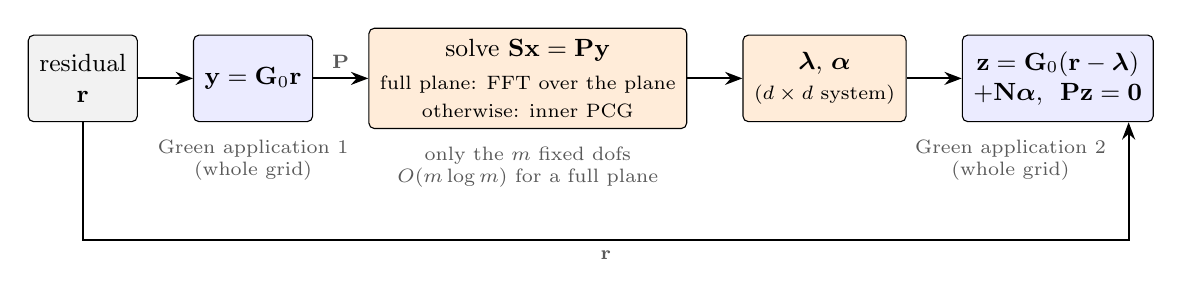
\begin{tikzpicture}[
      box/.style={draw, rounded corners=2pt, align=center, minimum height=11mm, inner sep=4pt, font=\small},
      grid/.style={box, fill=blue!8},
      wall/.style={box, fill=orange!15},
      arr/.style={-{Stealth[length=2.2mm]}, thick},
      lab/.style={font=\scriptsize, text=black!65, align=center}]
    \node[box, fill=black!5] (r) {residual\\ $\mathbf{r}$};
    \node[grid, right=7mm of r] (g1) {$\mathbf{y} = \mathbf{G}_0\mathbf{r}$};
    \node[wall, right=7mm of g1] (s) {solve $\mathbf{S}\mathbf{x} = \mathbf{P}\mathbf{y}$\\[1pt]
      \scriptsize full plane: FFT over the plane\\[-1pt] \scriptsize otherwise: inner PCG};
    \node[wall, right=7mm of s] (la) {$\boldsymbol{\lambda}$, $\boldsymbol{\alpha}$\\ \scriptsize ($d\times d$ system)};
    \node[grid, right=7mm of la] (g2) {$\mathbf{z} = \mathbf{G}_0(\mathbf{r} - \boldsymbol{\lambda})$\\ $+ \mathbf{N}\boldsymbol{\alpha}$,
      $\ \mathbf{P}\mathbf{z} = \mathbf{0}$};
    \draw[arr] (r) -- (g1);
    \draw[arr] (g1) -- node[above, lab] {$\mathbf{P}$} (s);
    \draw[arr] (s) -- (la);
    \draw[arr] (la) -- (g2);
    \draw[arr] (r.south) -- ++(0,-15mm) -| node[pos=0.25, below, lab] {$\mathbf{r}$} ($(g2.south)+(9mm,0)$);
    \node[lab, below=1mm of g1] {Green application 1\\ (whole grid)};
    \node[lab, below=1mm of g2, xshift=-6mm] {Green application 2\\ (whole grid)};
    \node[lab, below=1mm of s] {only the $m$ fixed dofs\\ $O(m\log m)$ for a full plane};
  \end{tikzpicture}
  \caption{One application $\mathbf{z} = \mathbf{M}_{\mathrm{GD}}\mathbf{r}$ of the corrected Green. Blue: operations on the
  whole grid, orange: operations on the fixed dofs only. With a full clamped plane the orange part costs nothing
  compared to the blue one.}
  \label{fig:flow}
\end{figure}

\paragraph{Inexact inner CG} (\texttt{run\_inexact.sh}; beam with 4 holes, $n_H = 32\to256$). $\mathbf{S}$ is applied
matrix-free, one Green application per product; $\operatorname{cond}(\mathbf{S}) \propto 1/h$.
\begin{itemize}
  \item There is a sharp threshold. Inner tolerance $10^{-8}$ (plain inner CG) or $10^{-6}$ (preconditioned, below)
        gives exactly the outer count of the direct solve (58 on every mesh). Looser solves make
        $\mathbf{M}_{\mathrm{GD}}$ a changing, non-symmetric operator and plain outer CG breaks down (hundreds to more
        than 5000 iterations, or no convergence). A warm start does not help.
  \item The solution stays correct whenever the outer CG converges, since $\mathbf{P}\mathbf{z} = \mathbf{0}$ is imposed.
  \item Plain inner CG needs $25\to63$ steps per outer iteration ($\times\sqrt2$ per refinement).
\end{itemize}

\begin{figure}[htbp]
  \centering
  \includegraphics[width=\textwidth]{inexact_study.png}
  \caption{Inexact inner solve of $\mathbf{S}$ (2D cantilever with holes). Outer CG iterations against the inner
  tolerance and against a fixed number of inner steps; total Green applications of the cheapest variant that keeps the
  direct outer count; compliance error. Open markers: no convergence within 5000 outer iterations.}
  \label{fig:inexact}
\end{figure}

\paragraph{Full grid planes: $\mathbf{S}$ is block-circulant.} $\mathbf{G}_0$ is translation-invariant. If the fixed
set is a complete grid plane (line in 2D) through the periodic cell, $\mathbf{S}$ inherits the invariance along the plane
and is diagonalized by the FFT over the plane. Each in-plane wave number $\boldsymbol{\xi}_{\parallel}$ gives a
$d\times d$ block, which by the projection-slice theorem is
\[
  \hat{\mathbf{S}}(\boldsymbol{\xi}_{\parallel}) = \frac{1}{N_{\perp}} \sum_{\xi_{\perp}} \hat{\mathbf{G}}_0(\boldsymbol{\xi}_{\parallel}, \xi_{\perp}).
\]
In practice the kernel is the response to a unit force at one plane node ($d$ Green applications), FFT'd over the plane
(Fig.~\ref{fig:symbol}). Fig.~\ref{fig:sets} sketches which fixed sets allow this.

\begin{figure}[htbp]
  \centering
  \includegraphics[width=\textwidth]{fixed_sets.pdf}
  \caption{Fixed sets on a periodic grid and the solve of $\mathbf{S}$ they allow. (a) A clamp on the solid face only:
  $\mathbf{S}$ is not circulant. (b) The same clamp continued through the void over the whole periodic cell: the void
  has zero stiffness, so the problem does not change, but $\mathbf{S}$ becomes block-circulant and is inverted exactly by
  an FFT along the line. (c) Parallel full lines: still exact. (d) Perpendicular lines: two families; inner PCG with each
  family inverted by its FFT, the crossing nodes in both.}
  \label{fig:sets}
\end{figure}

\begin{figure}[htbp]
  \centering
  \includegraphics[width=\textwidth]{wall_symbol.pdf}
  \caption{The wall FFT on real data (one full clamp line, isotropic reference). Left: the kernel of $\mathbf{S}$, the
  response along the line to a unit force at one line node (32, 64, 128 nodes on the line collapse). Right: the
  eigenvalues of its $2\times2$ symbol per wave number decay like $1/\xi$, hence $\operatorname{cond}\mathbf{S}\sim 1/h$
  and the growth of plain inner CG; inverting the symbol block by block is exact for every $\xi$.}
  \label{fig:symbol}
\end{figure}
\begin{itemize}
  \item \textbf{Clamp the plane through the void.} A clamp on the solid face only is not a full plane. Fixing also the
        void nodes on that plane does not change the problem (zero stiffness there); the compliance agrees to
        $5\times10^{-14}$.
  \item The solve $\mathbf{S}^{-1}\mathbf{g}$ is then one forward and one inverse FFT over the plane and a $d\times d$
        solve per wave number: no assembly, $O(m)$ memory, $O(m\log m)$ work, $d$ Green applications of setup.
        $\|\mathbf{S}\hat{\mathbf{S}}^{-1}\mathbf{g} - \mathbf{g}\|/\|\mathbf{g}\| = 10^{-14}$.
  \item Cantilever, $n_H = 32\to256$: 58 outer iterations and 118 Green applications in total on every mesh (dense:
        182 $\to$ 630 including assembly).
  \item \textbf{Several parallel planes} stay diagonal in $\boldsymbol{\xi}_{\parallel}$, with a
        $(p\,d)\times(p\,d)$ block for $p$ planes; also exact (two lines in 2D: $10^{-15}$).
\end{itemize}

\paragraph{Perpendicular planes (all faces of a box).} The crossings break the invariance; no exact FFT inverse.
Inner PCG with a block-Jacobi preconditioner over the \emph{families} of parallel planes, each inverted exactly by its
FFT symbol, works if the crossing nodes belong to \emph{both} families (overlapping additive Schwarz, contributions
summed). Giving them to one family only makes it worse than no preconditioner. Square with 4 holes, all four faces
clamped through the void (\texttt{box\_clamp\_study.py}), $N = 32\to256$:

\begin{center}
\small
\begin{tabular}{lcccc}
  \toprule
  solve of $\mathbf{S}$ & outer its & inner steps / outer & $\operatorname{cond}$ & Green apps, $N=256$ \\
  \midrule
  dense (assembled)              & 28--30 & --            & --                 & 4404 \\
  inner CG, $10^{-8}$            & 28--30 & 32 $\to$ 75   & 60 $\to$ 489       & 2545 \\
  inner PCG, per-line FFT, $10^{-6}$ & 28--30 & 18 $\to$ 20 & 22                & 734 \\
  inner PCG, family FFT, $10^{-6}$   & 28--30 & 10 $\to$ 13 & 4.7 $\to$ 11      & 492 \\
  family FFT once, no iteration  & 39 $\to$ 76 & --        & --                 & 162 \\
  \bottomrule
\end{tabular}
\end{center}
Two parallel lines on the same square: FFT exact, 31 outer iterations, 68 Green applications on every mesh
(Fig.~\ref{fig:box2d}).

\begin{figure}[htbp]
  \centering
  \includegraphics[width=\textwidth]{box_clamp_study.png}
  \caption{2D square with holes, fixed full lines through the void. Left: two parallel lines, total cost; the FFT
  solve is exact and costs 68 Green applications on every mesh. Middle and right: all four faces; inner PCG with the
  family FFT blocks needs 10--13 inner steps, against 32--75 for plain inner CG.}
  \label{fig:box2d}
\end{figure}

\paragraph{3D: clamped plane} (\texttt{plane\_clamp\_3D.py}, \texttt{run\_plane\_3D.sh}). Cantilever
$1\times0.2\times0.2$, void 0.05, uniform shear on the right face, clamped at the left face; the clamp plane runs
through the whole periodic cell and $\mathbf{S}$ is inverted by a 2D FFT over the plane, a $3\times3$ block per wave-number
pair, kernel from 3 Green applications (Fig.~\ref{fig:planes3d}, left). $\|\mathbf{S}\hat{\mathbf{S}}^{-1}\mathbf{g} - \mathbf{g}\|/\|\mathbf{g}\| \le
1.6\times10^{-15}$ on every mesh; all variants give the same compliance (to $10^{-10}$).

\begin{center}
\small
\begin{tabular}{lcccc}
  \toprule
  $n_H$ (grid) & 4 ($22\cdot6^2$) & 8 ($44\cdot12^2$) & 16 ($88\cdot24^2$) & 32 ($176\cdot48^2$) \\
  \midrule
  fixed dofs, full plane / solid face & 108 / 75 & 432 / 243 & 1728 / 867 & 6912 / 3267 \\
  outer its, plain Green $\mathbf{M}_{\mathrm{G}}$ & 54 & 65 & 78 & 102 \\
  outer its, $\mathbf{M}_{\mathrm{GD}}$ (any solve of $\mathbf{S}$) & 41 & 42--43 & 42--43 & 43 \\
  \midrule
  Green apps, dense $\mathbf{S}$, solid face & 159 & 329 & 953 & 3355 \\
  Green apps, dense $\mathbf{S}$, full plane & 192 & 520 & 1816 & 7000 \\
  Green apps, inner CG $10^{-8}$ (steps / outer) & 724 (15) & 1000 (21) & 1301 (28) & 1718 (37) \\
  Green apps, 2D FFT over the plane & 87 & 91 & 91 & 91 \\
  \bottomrule
\end{tabular}
\end{center}
With the FFT the corrected Green costs exactly two Green applications per iteration plus 3 for the setup. At
$n_H = 32$ that is 91 Green applications against 7000 for the dense $\mathbf{S}$ (207\,s of assembly, a 380\,MB matrix)
and 103 for the plain Green, which needs 102 iterations against 43, and its count keeps growing under refinement
(Fig.~\ref{fig:plane3d}).

\begin{figure}[htbp]
  \centering
  \includegraphics[width=0.95\textwidth]{planes_3D.pdf}
  \caption{3D fixed sets. Left: the cantilever's clamp plane continued through the void over the whole cell; one family,
  exact 2D FFT. Right: a cube clamped on all faces: three families of two parallel planes, inner PCG.}
  \label{fig:planes3d}
\end{figure}

\begin{figure}[htbp]
  \centering
  \includegraphics[width=0.9\textwidth]{plane_clamp_3D.png}
  \caption{3D cantilever with the clamp plane inverted by a 2D FFT. Left: outer CG iterations, plain against corrected
  Green. Right: total Green applications of the corrected Green for each solve of $\mathbf{S}$.}
  \label{fig:plane3d}
\end{figure}

\paragraph{3D: cube clamped on all six faces} (\texttt{box\_clamp\_3D.py}, \texttt{run\_box\_3D.sh}). Cube with 8
spherical holes, void buffer, body force; the six face planes through the whole cell, i.e.\ 3 families of 2 parallel
planes, each family inverted exactly by a 2D FFT ($6\times6$ block per wave-number pair), edges and corners in every
family that contains them. The family preconditioner alone has a relative error of 0.58, 0.41, 0.28 and 0.20 at $N = 8$, 16, 32 and 64.

\begin{center}
\small
\begin{tabular}{lcccc}
  \toprule
  $N$ (grid) & 8 ($10^3$) & 16 ($18^3$) & 32 ($36^3$) & 64 ($72^3$) \\
  \midrule
  fixed dofs $m$ & 1464 & 5208 & 22056 & 90744 \\
  outer its, plain Green $\mathbf{M}_{\mathrm{G}}$ & 23 & 44 & 69 & 94 \\
  outer its, $\mathbf{M}_{\mathrm{GD}}$ (any solve of $\mathbf{S}$) & 20 & 29 & 33--34 & 33--34 \\
  outer its, family FFT once (no iteration) & 21 & 42 & 70 & 193 \\
  inner steps / outer: plain CG $10^{-8}$ & 26 & 37 & 50 & 68 \\
  inner steps / outer: PCG family FFT $10^{-6}$ & 14 & 15 & 16 & 18.5 \\
  \midrule
  Green apps (setup + solve), dense $\mathbf{S}$ & 1506 & 5268 & 22124 & -- \\
  Green apps (setup + solve), inner PCG family FFT & 433 & 599 & 745 & 837 \\
  Green apps, plain Green & 24 & 45 & 70 & 95 \\
  \bottomrule
\end{tabular}
\end{center}
At $N = 64$ the dense $\mathbf{S}$ would need 66\,GB. Counted in Green applications, the plain Green is cheapest, but
here one stiffness application costs about 130 Green applications (1.78\,s against 14\,ms at $N = 64$, CPU). The work
is then set by the outer iterations: 34 for the corrected Green against 94 for the plain one
(Figs.~\ref{fig:box3d} and~\ref{fig:box3ddef}).

\begin{figure}[htbp]
  \centering
  \includegraphics[width=\textwidth]{box_clamp_3D.png}
  \caption{Cube clamped on all six faces. Left: outer CG iterations; the corrected Green (any solve of $\mathbf{S}$)
  stays at 34, the family FFT applied once without iterating does not. Middle: total Green applications. Right: inner
  steps per outer iteration, plain inner CG against inner PCG with the family 2D FFTs.}
  \label{fig:box3d}
\end{figure}

\begin{figure}[htbp]
  \centering
  \includegraphics[width=\textwidth]{box_clamp_3D_deformation_N32.png}
  \caption{Cube clamped on all six faces, $N = 32$: the displacement on three cuts (magnified; the clamped faces do not
  move), and the outer CG convergence. The inner-PCG curve lies on the dense-$\mathbf{S}$ curve.}
  \label{fig:box3ddef}
\end{figure}

\paragraph{Removing the crossing nodes does not decouple perpendicular lines.} $\mathbf{G}_0$ is global, so two
perpendicular lines are coupled along their whole length, not only at the crossing. 2D, with the exact (dense)
inverse of each family's own block $\mathbf{D}$: $\|\mathbf{S}_{VH}\|/\|\mathbf{D}\| = 0.27$ with the crossing kept and
0.26 with it removed (one corner, $N = 32$), and $\operatorname{eig}(\mathbf{D}^{-1}\mathbf{S}) \in [0.18, 1.83]$ against
$[0.26, 1.74]$. The block-diagonal inverse stays a preconditioner, not an exact solve, and removing the crossing also makes
each line incomplete, so its FFT is no longer exact either.

\paragraph{Second level on the crossing patches.} The bad modes of the family preconditioner $\mathbf{M}^{-1}$ (the
overlapping families) sit at the crossings, but they extend a few nodes along the lines. Let $\mathbf{Z}$ select
the fixed dofs within $k$ nodes of a crossing (a patch of fixed size, independent of $N$). Its block
$\mathbf{S}_{ZZ} = \mathbf{Z}^{\top}\mathbf{S}\mathbf{Z}$ is assembled once, one Green application per patch dof, and the
full columns $\mathbf{S}\mathbf{Z}$ are kept. With $\mathbf{Q} = \mathbf{Z}\mathbf{S}_{ZZ}^{-1}\mathbf{Z}^{\top}$, compare
\[
  \text{additive: } \mathbf{C}^{-1} = \mathbf{M}^{-1} + \mathbf{Q}, \qquad
  \text{balancing: } \mathbf{C}^{-1} = \mathbf{Q} + (\mathbf{I} - \mathbf{Q}\mathbf{S})\,\mathbf{M}^{-1}(\mathbf{I} - \mathbf{S}\mathbf{Q}).
\]
The balancing form is symmetric and, with $\mathbf{S}\mathbf{Z}$ stored, needs no Green application beyond the PCG's own
one per step. 2D square, all four faces clamped (\texttt{box\_clamp\_study.py}, \texttt{PATCH}, \texttt{PATCH\_MODE};
\texttt{run\_box\_patch.sh}, \texttt{box\_patch\_plot.py}), Figs.~\ref{fig:patchspec} and~\ref{fig:patchcost}:
\begin{itemize}
  \item The crossing node alone ($k = 0$) does nothing: cond 11 $\to$ 10 at $N = 256$.
  \item Additive patches lift $\lambda_{\min}$ but raise $\lambda_{\max}$ from 2 to 3; inner steps do not drop.
  \item Balancing patches keep $\lambda_{\max} \approx 1.3$--$1.4$ and lift $\lambda_{\min}$ to 0.4--0.6. cond goes from
        4.7--11 (families only, $N = 32\to256$) to 2.1--3.4 for $k = 2$ and 1.6--2.3 for $k = 8$. Inner steps per outer
        iteration drop from 10--12.7 to 6--8.6 ($k = 2$) and 4--7 ($k = 8$). The outer count (28--30) and the
        compliance are unchanged.
  \item The total cost gains less, because the patch is assembled: at $N = 256$, $k = 2$ gives 428 Green applications against
        492 for the families only, and $k \ge 8$ costs more than it saves. $k = 2$ to $4$ is the sweet spot here.
\end{itemize}

\begin{figure}[htbp]
  \centering
  \includegraphics[width=\textwidth]{box_patch_spectra.png}
  \caption{Second level on the crossing patches. (a) Sketch: the two families inverted by 1D FFTs, the patches around
  the crossings by a small dense solve. (b) Sorted eigenvalues of $\mathbf{C}^{-1}\mathbf{S}$ at $N = 128$: the family
  preconditioner leaves a few small eigenvalues (the corner modes) and $\lambda_{\max} = 2$; the balancing second level
  removes both ends. (c) cond($\mathbf{C}^{-1}\mathbf{S}$) against the mesh.}
  \label{fig:patchspec}
\end{figure}

\begin{figure}[htbp]
  \centering
  \includegraphics[width=\textwidth]{box_patch_cost.png}
  \caption{Inner PCG steps per outer iteration and total Green applications (including the assembly of the patch block)
  for the family preconditioner alone, with additive and with balancing patches of $\pm k$ nodes.}
  \label{fig:patchcost}
\end{figure}

\paragraph{Second level in 3D: edge strips.} In the cube the crossings are the 12 edge lines, each a full line
through the cell, so the patches become strips of $\pm k$ nodes along the edges and grow with $N$ (23\,328 dofs at
$N = 64$, $k = 2$): too large for a dense block or a stored $\mathbf{S}\mathbf{Z}$. The 4 parallel edges of one direction
are, however, translation-invariant along the edges, so their block is inverted exactly by a 1D FFT along them (setup:
one Green application per dof of a cross-section, 144--324, independent of $N$; residual $3\times10^{-15}$). The three
groups overlap near the corners and are summed with weights $1/\sqrt{\text{multiplicity}}$ (unweighted, the inner PCG
gets worse: 25 steps against 15). Without $\mathbf{S}\mathbf{Z}$, balancing costs two extra Green applications per inner
step (\texttt{box\_clamp\_3D.py PATCH=k}, \texttt{run\_box\_3D\_patch.sh}, Fig.~\ref{fig:box3d}):

\begin{center}
\small
\begin{tabular}{lcccc}
  \toprule
  $N$ & 8 & 16 & 32 & 64 \\
  \midrule
  inner steps / outer, families only & 14 & 15 & 16 & 18.5 \\
  inner steps / outer, + edge strips $\pm1$ / $\pm2$ & 8.9 / 9.8 & 9.8 / 9.9 & 13.3 / 11.7 & 16.9 / 16.5 \\
  Green apps total, families only & 433 & 599 & 745 & 837 \\
  Green apps total, + edge strips $\pm1$ / $\pm2$ & 888 / 1026 & 1251 / 1326 & 1843 / 1727 & 2287 / 2356 \\
  \bottomrule
\end{tabular}
\end{center}
The gain in inner steps (about a third on coarse meshes) fades under refinement (10\,\% at $N = 64$), and each step costs
three Green applications, so the total triples. In 3D the families-only preconditioner stays the method of choice.

\paragraph{The sub-block of the reference stiffness is not $\mathbf{S}^{-1}$.} $\mathbf{S}$ consists of the
fixed-dof rows and columns of $\mathbf{G}_0 = \mathbf{K}_0^{-1}$, but the inverse of a sub-block is not the sub-block of
the inverse. Block inversion gives
\[
  \mathbf{S}^{-1} = \mathbf{K}_{FF} - \mathbf{K}_{FI}\mathbf{K}_{II}^{-1}\mathbf{K}_{IF}
\]
(the Dirichlet-to-Neumann operator). The term $\mathbf{K}_{FI}\mathbf{K}_{II}^{-1}\mathbf{K}_{IF}$ is positive
semidefinite, so $\mathbf{K}_{FF} \ge \mathbf{S}^{-1}$ and $\operatorname{eig}(\mathbf{K}_{FF}\mathbf{S}) \ge 1$, with
equality only if the fixed dofs did not couple to the free ones. Inner PCG with
$\mathbf{K}_{FF} = \mathbf{P}\mathbf{K}_{\mathrm{ref}}\mathbf{P}$ (\texttt{INNER=kff}, \texttt{run\_box\_kff.sh},
\texttt{box\_kff\_plot.py}, Fig.~\ref{fig:kff}), 2D square with all four faces clamped:
$\operatorname{eig}(\mathbf{K}_{FF}\mathbf{S}) \in [1.0, 27 \to 219]$ for $N = 32\to256$. The condition number halves
against no preconditioner (27--217 against 60--489) but keeps growing like $1/h$. Inner steps drop from 24--54 to
18--40, against 10--12.7 for the family FFT. $\mathbf{K}_{FF}$ is a local stencil with bounded condition number (5 on one
line), while $\mathbf{S}^{-1}$ has a symbol $\sim|\xi|$; the missing coupling term carries that growth.

\begin{figure}[htbp]
  \centering
  \includegraphics[width=\textwidth]{box_kff.png}
  \caption{Inner solve of $\mathbf{S}$ preconditioned by $\mathbf{K}_{FF} = \mathbf{P}\mathbf{K}_{\mathrm{ref}}\mathbf{P}$,
  against no preconditioner and the family FFT. (a) Spectra at $N = 128$: $\mathbf{K}_{FF}$ lifts the bottom of the
  spectrum to 1 but leaves the $1/h$ spread. (b) Condition numbers. (c) Inner PCG steps per outer iteration.}
  \label{fig:kff}
\end{figure}

\paragraph{A local Schur complement on a strip.} $\mathbf{K}_{II}$ is $\mathbf{K}_{\mathrm{ref}}$ with the fixed dofs
struck out, so $\mathbf{K}_{II}^{-1}$ is the reference problem clamped on $F$, the corrected Green itself: the exact
formula is circular. $\mathbf{K}_{FI}$ only reaches the stencil neighbours of $F$, so we keep $\mathbf{K}_{II}$ only on a
strip $I_w$ of the free dofs within $w$ nodes of a fixed node, clamped at the strip's edge:
\[
  \mathbf{S}_w^{-1} = \mathbf{K}_{FF} - \mathbf{K}_{FI_w}\mathbf{K}_{I_wI_w}^{-1}\mathbf{K}_{I_wF},
  \qquad \mathbf{K}_{FF} = \mathbf{S}_0^{-1} \ge \mathbf{S}_w^{-1} \ge \mathbf{S}_\infty^{-1}.
\]
($\mathbf{K}_{\mathrm{ref}}$ assembled sparse by probing, $2p^2$ applications with a colouring of period $p \ge 3$; the
strip block factorized once; \texttt{INNER=strip STRIP\_W=}$w$, \texttt{run\_box\_strip.sh}, \texttt{box\_strip\_plot.py}.)
The full Schur complement of the periodic $\mathbf{K}_{\mathrm{ref}}$ annihilates the two translations (constants per
component on $F$) while $\mathbf{S}$ does not, so $\lambda_{\min}$ drops to 0 as $w$ grows; a balancing step on that
two-dimensional coarse space, $\mathbf{C}^{-1} = \mathbf{Q} + (\mathbf{I}-\mathbf{Q}\mathbf{S})\mathbf{S}_w^{-1}
(\mathbf{I}-\mathbf{S}\mathbf{Q})$, $\mathbf{Q} = \mathbf{B}(\mathbf{B}^\top\mathbf{S}\mathbf{B})^{-1}\mathbf{B}^\top$,
repairs it. On one line the symbols are $|\xi|$ (exact) and $|\xi|\coth(|\xi| w)$ (strip): the strip gets the high
frequencies right and overestimates the low ones by about $L/w$. The measurements agree (Fig.~\ref{fig:strip},
$N = 32, 64, 128$):
\begin{center}\small
\begin{tabular}{lrrr}
  \hline
  cond$(\mathbf{C}^{-1}\mathbf{S})$ & $N = 32$ & 64 & 128 \\
  \hline
  $\mathbf{K}_{FF}$ ($w = 0$) & 27 & 54 & 108 \\
  strip $w = 2$ px & 4.1 & 8.8 & 36 \\
  strip $w = 8$ px & 1.5 & 2.5 & 5.7 \\
  strip $w = N/16$ (fixed physical width) & 4.1 & 5.1 & 5.7 \\
  family FFT & 4.7 & 6.3 & 8.5 \\
  \hline
\end{tabular}
\end{center}
A fixed width in pixels still grows like $1/h$; a fixed physical width is nearly bounded and beats the family FFT
(10.3 against 11.7 inner steps at $N = 128$, outer count unchanged). The strip needs no full lines and no special
treatment of crossings or corners. Its price is a sparse solve on about $m w$ dofs: cheap in 2D, but in 3D a slab of
fixed physical thickness around every clamped face is a 3D sparse factorization of a sizeable part of the grid.

\begin{figure}[htbp]
  \centering
  \includegraphics[width=\textwidth]{box_strip.png}
  \caption{Inner solve of $\mathbf{S}$ preconditioned by the local Schur complement on a strip of width $w$ (balanced on
  the translations). (a) Fixed width in pixels. (b) Fixed physical width $w/N$. (c) Inner PCG steps.}
  \label{fig:strip}
\end{figure}

\paragraph{Making the pixels around a crossing void does not help either.} $\mathbf{S} = \mathbf{P}\mathbf{G}_0\mathbf{P}$
is built from the homogeneous reference only; it depends on which dofs are fixed, never on which pixels are solid or
void. Void changes $\mathbf{K}$, not $\mathbf{S}$. (That is also why clamping the void part of a plane is free: it
completes the fixed set without changing the physical problem.) An exact decoupling would need a reference problem
whose Green operator already satisfies the clamp on the box faces. Sine/cosine transforms give one for scalar problems and
for roller (symmetry) conditions in elasticity, but not for fully clamped elasticity, where the mixed derivatives couple
the parities of the displacement components.

\paragraph{Summary.}
\begin{center}
\small
\begin{tabular}{p{0.38\textwidth}p{0.55\textwidth}}
  \toprule
  fixed set & solve of $\mathbf{S}$ \\
  \midrule
  one plane or parallel planes, through the whole cell & FFT over the plane: exact, essentially free \\
  perpendicular planes (box faces) & inner PCG, family FFT blocks, overlap at crossings: $\approx 13$ steps;
  with a balancing second level on crossing patches ($\pm2$--$4$ nodes): 6--9 steps \\
  arbitrary (holes, partial faces, points) & inner PCG (tolerance $\le10^{-6}$), or dense if $m$ is small \\
  \bottomrule
\end{tabular}
\end{center}


\section*{Remarks}

\begin{itemize}
  \item This is the \emph{capacitance matrix method} of fast Poisson solvers on irregular domains (Buzbee, Dorr, George
        and Golub 1971; Proskurowski and Widlund 1976), used here as a preconditioner rather than as a direct solver.
  \item \textbf{Cost of the setup} grows with $m$: $m$ Green applications and a dense $(m+d)$ factorization. That is
        cheap for a clamped face in 2D ($m = 2(n_H+1)$). For large $m$ see the section above.
  \item \textbf{Prescribed nonzero values} change only the right-hand side (lifting), not $\mathbf{M}_{\mathrm{GD}}$.
  \item \textbf{Materials stiffer than the reference} ($\mathbb{C}_q > \mathbb{C}_0$, e.g.\ a stiff layer) still give
        $\lambda_{\max} > 1$; the correction removes only the effect of the fixed dofs.
\end{itemize}

\section*{Conclusions}

\begin{enumerate}
  \item \textbf{The corrected Green works.} It is the exact inverse of the constrained reference problem, so
        $\lambda_{\max} = 1$ and the outer CG count is mesh-independent: 2D cantilever 30--32 (plain Green 46--94),
        3D cantilever 41--43 (54--102), 3D cube clamped on all faces 34 (94). Each iteration costs 2 Green applications
        plus one solve with $\mathbf{S}$, of size $m$ = number of fixed dofs.
  \item \textbf{The dense $\mathbf{S}$ does not scale.} It needs $m$ Green applications to assemble, $8m^2$ bytes, and
        $m^3$ flops to factorize. That is fine in 2D but infeasible in 3D (one face at $N = 128$: 20\,GB; six faces at
        $N = 64$: 66\,GB).
  \item \textbf{An inexact inner CG works only if it is accurate.} There is a sharp threshold: inner tolerance
        $10^{-8}$ for plain inner CG, or $10^{-6}$ with the FFT preconditioner. Below it the outer CG is unchanged;
        above it the outer CG breaks down. Plain inner CG slows down under refinement
        ($\operatorname{cond}\mathbf{S} \sim 1/h$).
  \item \textbf{Key trick: clamp the full plane through the void.} Zero stiffness, so the problem is unchanged, but
        $\mathbf{S}$ becomes circulant and is solved exactly by an FFT over the plane: no assembly, $O(m)$ memory,
        $d$ Green applications of setup. This holds for one plane and for parallel planes. 3D cantilever,
        $n_H = 32$: 91 Green applications in total against 7000 for the dense $\mathbf{S}$.
  \item \textbf{Perpendicular planes (box, all faces): no exact FFT.} Inner PCG with each family of parallel planes
        inverted by its FFT, crossing nodes in both families: 10--13 inner steps in 2D and 14--18.5 in 3D, slowly growing
        with $N$; the outer count is identical to the dense solve.
  \item \textbf{What does not remove the crossing problem:} removing the crossing node (the lines stay coupled along
        their whole length), making the pixels around it void ($\mathbf{S}$ sees only the reference material), and a
        correction on the crossing node only.
  \item \textbf{A second level on patches around the crossings} helps in 2D, in its balancing form with patches of
        $\pm2$--$4$ nodes: cond 11 $\to$ 3.4, inner steps 12.7 $\to$ 8.6, about 13\,\% less total cost. In 3D the patches
        become strips along the edges, the savings fade under refinement, and each step costs three Green applications:
        not worth it.
  \item \textbf{Cost perspective.} One stiffness application costs about 130 Green applications in our CPU
        implementation. The outer iteration count dominates; the inner solve with $\mathbf{S}$ is nearly free once it
        uses FFTs.
\end{enumerate}

\begin{center}
\small
\begin{tabular}{p{0.38\textwidth}p{0.55\textwidth}}
  \toprule
  fixed set & solve of $\mathbf{S}$ \\
  \midrule
  one plane or parallel planes (clamped ends) & clamp through the void, FFT over the plane: exact, essentially free \\
  perpendicular planes (box faces) & inner PCG with the family FFTs, crossing nodes in both families (in 2D plus a
  balancing patch of $\pm2$ nodes) \\
  arbitrary supports (points, partial faces, holes) & dense $\mathbf{S}$ if $m$ is small, otherwise inner CG / PCG with
  tolerance $\le 10^{-6}$ \\
  \bottomrule
\end{tabular}
\end{center}

\noindent\textbf{In one sentence:} the bottleneck of the dense direct solve disappears if the clamp is made a full grid
plane by extending it through the void. $\mathbf{S}$ is then solved exactly by an FFT, and only perpendicular planes
still need a short inner iteration of about 15 steps.

\end{document}
